\documentclass[letterpaper,11pt]{article}

\usepackage{geometry}
\usepackage{pslatex}
\usepackage{fancyhdr}
\usepackage{graphicx}
\usepackage{color}
\usepackage{tikz}
\usepackage{setspace}
\usepackage{amssymb}

\geometry{ margin = 1.0in }

\pagestyle{fancy}
\lhead{{\bf Lecture 41}}
\chead{{\bf CMPSC 465 Fall 2020}}
\rhead{{\bf Mingfu Shao}}

\setlength\parindent{0em}
\setlength\parskip{8pt}
%\setlength{\fboxsep}{6pt}

\usepackage{amsthm}
\newtheoremstyle{mytheorem}
  {\parskip} % Space above
  {0em} % Space below
  {} % Body font
  {} % Indent amount
  {\bfseries} % Theorem head font
  {.} % Punctuation after theorem head
  {.5em} % Space after theorem head
  {} % Theorem head spec (can be left empty, meaning `normal')

\theoremstyle{mytheorem}
\newtheorem{definition}{Definition}
\newtheorem{property}{Property}
\newtheorem{claim}{Claim}
\newtheorem{fact}{Fact}
\newtheorem{corollary}{Corollary}

% for algorithms
\newcommand{\aaa}[1]{\hspace{0.65cm}\parbox[t]{15.3cm}{#1}}
\newcommand{\aab}[1]{\hspace{1.15cm}\parbox[t]{15.0cm}{#1}}
\newcommand{\aac}[1]{\hspace{1.65cm}\parbox[t]{15.0cm}{#1}}
\newcommand{\aad}[1]{\hspace{2.15cm}\parbox[t]{15.0cm}{#1}}
\newcommand{\aae}[1]{\hspace{2.65cm}\parbox[t]{15.0cm}{#1}}
\newcommand{\aaf}[1]{\hspace{3.15cm}\parbox[t]{15.0cm}{#1}}
\newcommand{\aaA}[2]{\hspace{0.5cm} {\tikz[overlay] \draw (0.1, -0.1) -- (0.1, #1 * -1.5em + 0.6em);} \parbox[t]{15.0cm}{#2}}
\newcommand{\aaB}[2]{\hspace{1.0cm} {\tikz[overlay] \draw (0.1, -0.1) -- (0.1, #1 * -1.5em + 0.6em);} \parbox[t]{15.0cm}{#2}}
\newcommand{\aaC}[2]{\hspace{1.5cm} {\tikz[overlay] \draw (0.1, -0.1) -- (0.1, #1 * -1.5em + 0.6em);} \parbox[t]{15.0cm}{#2}}
\newcommand{\aaD}[2]{\hspace{2.0cm} {\tikz[overlay] \draw (0.1, -0.1) -- (0.1, #1 * -1.5em + 0.6em);} \parbox[t]{15.0cm}{#2}}
\newcommand{\aaE}[2]{\hspace{2.5cm} {\tikz[overlay] \draw (0.1, -0.1) -- (0.1, #1 * -1.5em + 0.6em);} \parbox[t]{15.0cm}{#2}}
\newcommand{\xxx}{\par\vspace{0.1cm}}

\begin{document}

\section*{NP-complete and NP-hard}

\subsection*{Polynomial-Time Reduction Revisit}

Polynomial-time reduction can be used in two different ways. Suppose we have $X\le_p Y$.
\vspace*{-\topsep}
\begin{enumerate}
\item If we know an algorithm to solve $Y$, then we know how to solve $X$. In this way
we are making use of an (existing) algorithm for $Y$ to solve a (new) problem $X$. Such an example
is we use the maximum flow problem~(problem $Y$) to solve the bipartite maximum matching problem~(problem $X$).
\item If we know problem $X$ is \emph{hard}, then we know that problem $Y$ is \emph{hard}. 
This is because $X\le_p Y$ means that $Y$ is at least as hard as $X$, as any algorithm of $Y$ can be used to solve $X$.
In this way, we are making use of an (existing) hard problem $X$
to prove that a (new) problem $Y$ is hard.  Below we will formally define ``hard''.
Informally, it means a polynomial-time algorithm does not exist~(unless P{}~$=${}~NP).
\end{enumerate}


\subsection*{NP-complete}

\begin{definition}[NP-complete]
Let $X$ be a decision problem. We say $X$ is NP-complete, if $X$ is in NP, and for every problem $X'$ in NP, we have $X'\le_p X$.
\end{definition}

NP-complete problems are the ``hardest'' problems in NP. It's not obvious that
NP-complete problems even exist.  
Thanks to the pioneers of computer science: in 1971 Cook and Levin proved the first
NP-complete problem by showing that the circuit satisfiability problem is NP-complete.
This builds the foundation of complexity theory.

One side of application of NP-complete relates to the connection between P and NP.
Clearly, P is a subset of NP, i.e., P{}~$\subset${}~NP.
But is the case that P{}~$\neq${}~NP~(i.e., P is a strict subset of NP),
or P{}~$=${}~NP?  This question remains open,
and is perhap \emph{the} most important open question in computer science.
(It is also one of the seven Millennium Prize Problems selected by the Clay Mathematics Institute.)
The existence of NP-complete problems gives a way to prove that P{}~$=${}~NP, by just showing
one NP-complete problem is polynomial-time solvable. This is easy to understand: NP-complete
problems are the hardest problems in NP; if one of them is polynomial-time solvable,
then every problem must be polynomial-time solvable. We formally state it and prove it below.

\begin{claim}
Let $X$ be a NP-complete problem. If $X$ is in P, then we have P{}~$=${}~NP.
\end{claim}

\emph{Proof.} 	
In order to show P{}~$=${}~NP, we only need to prove NP{}~$\subset${}~P, as we already have P{}~$\subset${}~NP. 
Let $X'$ be an arbitrary problem in NP.  
Since $X$ is NP-complete, by definition, we know that $X'\le_p X$. Because
$X$ is in P, then we have that $X'$ is in P as well~(see Fact~1 in Lecture~40).
This proves that NP{}~$\subset${}~P, as $X'$ is arbitrary.  \qed

Above claims suggests the two possible cases between P, NP, and NPC---here we use ``NPC''
to represent the set of all NP-complete problems. See Figure~\ref{fig:PvsNP}.

\begin{figure}[!h]
\centering{

\tikzset{every picture/.style={line width=0.75pt}} %set default line width to 0.75pt        

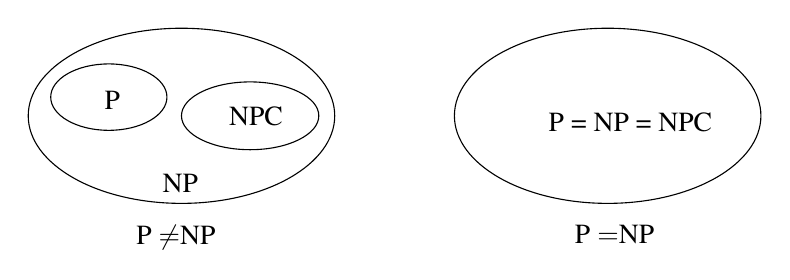
\begin{tikzpicture}[x=0.5pt,y=0.5pt,yscale=-1,xscale=1]
%uncomment if require: \path (0,174); %set diagram left start at 0, and has height of 174

%Shape: Ellipse [id:dp7503072037089505] 
\draw   (7.75,74.5) .. controls (7.75,39.55) and (57.33,11.21) .. (118.5,11.21) .. controls (179.67,11.21) and (229.25,39.55) .. (229.25,74.5) .. controls (229.25,109.45) and (179.67,137.79) .. (118.5,137.79) .. controls (57.33,137.79) and (7.75,109.45) .. (7.75,74.5) -- cycle ;
%Shape: Ellipse [id:dp9197904806155399] 
\draw   (24,61) .. controls (24,47.75) and (42.8,37) .. (66,37) .. controls (89.2,37) and (108,47.75) .. (108,61) .. controls (108,74.25) and (89.2,85) .. (66,85) .. controls (42.8,85) and (24,74.25) .. (24,61) -- cycle ;
%Shape: Ellipse [id:dp11719807374253621] 
\draw   (118.5,74.5) .. controls (118.5,60.97) and (140.72,50) .. (168.13,50) .. controls (195.53,50) and (217.75,60.97) .. (217.75,74.5) .. controls (217.75,88.03) and (195.53,99) .. (168.13,99) .. controls (140.72,99) and (118.5,88.03) .. (118.5,74.5) -- cycle ;
%Shape: Ellipse [id:dp5090440012854042] 
\draw   (315.75,74.5) .. controls (315.75,39.55) and (365.33,11.21) .. (426.5,11.21) .. controls (487.67,11.21) and (537.25,39.55) .. (537.25,74.5) .. controls (537.25,109.45) and (487.67,137.79) .. (426.5,137.79) .. controls (365.33,137.79) and (315.75,109.45) .. (315.75,74.5) -- cycle ;


% Text Node
\draw (382,70) node [anchor=north west][inner sep=0.75pt]   [align=left] {P = NP = NPC};
% Text Node
\draw (61,55) node [anchor=north west][inner sep=0.75pt]   [align=left] {P};
% Text Node
\draw (151,66) node [anchor=north west][inner sep=0.75pt]   [align=left] {NPC};
% Text Node
\draw (103,115) node [anchor=north west][inner sep=0.75pt]   [align=left] {NP};
% Text Node
\draw (84,151.5) node [anchor=north west][inner sep=0.75pt]   [align=left] {P $\displaystyle \neq $NP};
% Text Node
\draw (401,151.5) node [anchor=north west][inner sep=0.75pt]   [align=left] {P $\displaystyle =$NP};


\end{tikzpicture}

}
\caption{Two possibilities among P, NP, and NPC.}
\label{fig:PvsNP}
\end{figure}

\vspace*{-\topsep}
\begin{enumerate}
\item P{}~$\neq${}~NP. In this case, we must have P{}~$\cap${}~NPC{}~$=\emptyset$. This is
because otherwise, if there exists a problem $X\in \textrm{ P } \cap \textrm{ NPC}$, P will be equal to NP according to above Claim). 
\item P{}~$=${}~NP. In this case, we must have P{}~$=${}~NP{}~$=${}~NPC. 
This is because in this case \emph{any} two problems $X$ and $Y$ in NP~(and therefore in P)
must satisfy that $X\le_p Y$ and $Y\le_p X$, as both $X$ and $Y$ can be solved in polynomial-time.
This proves that every problem in NP is NP-complete.
\end{enumerate}

Another side of application of NP-complete problems is to use existint NP-complete problems
to prove new problems are NP-complete~(i.e., hard). This is based on the following claim.

\begin{claim}
Let $X$ be a problem in NP. If there exists an NP-complete problem $Y$ such that $Y\le_p X$,
we we have $X$ is NP-complete.
\end{claim}

This is easy to understand: $Y$ is NP-complete, i.e., it is (one of) the hardest problem
in NP; of course $Y$ is at least as hard as $X$ because $X$ is in NP.
Now we have $Y\le_p X$, i.e., $X$ is at least as hard as $Y$. Combined, $X$ is (one of) the
hardest problem in NP as well. Below we give a formal proof.

\emph{Proof.} Let $X'$ an arbitrary problem in NP. Since problem $Y$ is NP-complete,
by definition, we have $X' \le_p Y$. Since $Y\le_p X$, we must have that $X'\le X$.
(Here we use the property that the polynomial-time reduction is transitive.)
Combining that $X$ is in NP, we know that $X$ is NP-complete.\qed

Above Claim suggest a procedure to prove that a decision problem $X$ is NP-complete.
\vspace*{-\topsep}
\begin{enumerate}
\item show that $X$ is in NP;
\item pick an existing NP-complete problem $Y$;
\item show that $Y$ is polynomial-time reducible to $X$. 
\end{enumerate}

Using above procedure, lots of problems have been proved to be NP-complete.
These includes the 3SAT problem, the decision-version of the vertex cover problem, i.e., $VC(G,k)$.
Other well-known NP-complete problems include, the decision-version of independenet set problem,
the Hamiltonian path problem, 
the Hamiltonian cycle problem, 
3D matching problem, $k$-coloring problem when $k\ge 3$, the subset-sum problem, decision-version of TSP~(traveling salesman problems), etc.
Below we give some details for the independent set problem.

\subsection*{The Independent Set Problem}

An \emph{independent set} of an undirected graph $G = (V, E)$
is a subset of vertices $V_1\subset V$ satisfying that no two vertices in it is connected by an edge, i.e.,
for any $u,v\in V_1$, we have $(u,v)\not\in E$. We define two versions of the independent set problem.
\vspace*{-\topsep}
\begin{enumerate}
\item optimization-version: given an undirected graph $G = (V, E)$, to seek an independent set $V_1$ of $G$ such that $V_1$ is maximized; we denote this problem as $IS(G)$;
\item decision-version: given an undirected graph $G = (V, E)$ and integer $k\ge 0$, to decide if there exists an independent set $V_1$ of $G$ such that $|V_1| \ge k$;
we denote this problem as $IS(G,k)$.
\end{enumerate}

There is a simple connection between independent set and vertex cover, stated below. Can you spot why?
See Figure~\ref{fig:is} for an example.

\begin{claim}
Let $G = (V, E)$ be an undirected graph. We have $V_1\subset V$ is an independent set of $G$ if and only if $V\setminus V_1$ is a vertex cover of $G$.
\end{claim}

\begin{figure}[!h]
\centering{

\tikzset{every picture/.style={line width=0.75pt}} %set default line width to 0.75pt        

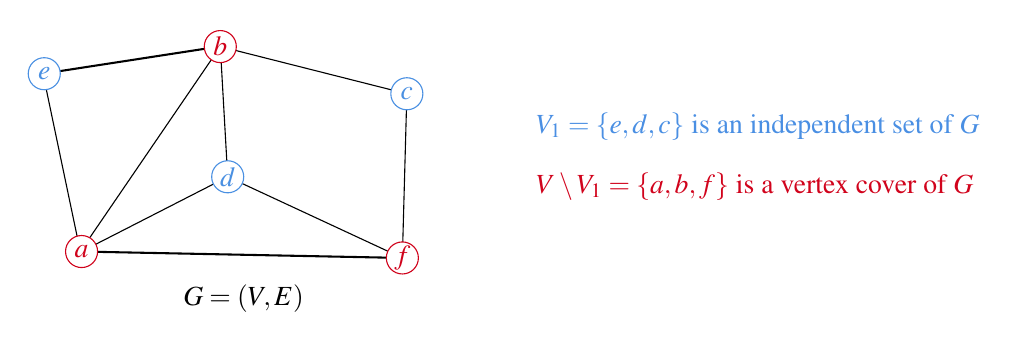
\begin{tikzpicture}[x=0.5pt,y=0.5pt,yscale=-1,xscale=1]
%uncomment if require: \path (0,207); %set diagram left start at 0, and has height of 207

%Straight Lines [id:da7485926733039977] 
\draw    (144.6,14.97) -- (43.43,163.09) ;
%Straight Lines [id:da4575120980127291] 
\draw [color={rgb, 255:red, 0; green, 0; blue, 0 }  ,draw opacity=1 ][line width=0.75]    (16.46,34.58) -- (143.69,14.97) ;
%Straight Lines [id:da9165715401778428] 
\draw    (16.46,34.58) -- (43.43,163.09) ;
%Straight Lines [id:da994182434786223] 
\draw [color={rgb, 255:red, 0; green, 0; blue, 0 }  ,draw opacity=1 ][line width=0.75]    (44.34,163.09) -- (276.17,167.73) ;
%Straight Lines [id:da9750224919648968] 
\draw    (149.95,109.07) -- (276.17,167.73) ;
%Straight Lines [id:da24348552449211425] 
\draw    (144.6,14.97) -- (149.95,109.07) ;
%Straight Lines [id:da16705340438790406] 
\draw    (144.6,14.97) -- (279.42,49.07) ;
%Straight Lines [id:da08663700279220432] 
\draw    (279.42,49.07) -- (276.17,167.73) ;
%Straight Lines [id:da4151454155794566] 
\draw    (149.95,109.07) -- (44.34,163.09) ;
%Shape: Ellipse [id:dp9133580928774087] 
\draw  [color={rgb, 255:red, 74; green, 144; blue, 226 }  ,draw opacity=1 ][fill={rgb, 255:red, 255; green, 255; blue, 255 }  ,fill opacity=1 ] (5.79,34.58) .. controls (5.79,28.18) and (10.97,23) .. (17.37,23) .. controls (23.76,23) and (28.95,28.18) .. (28.95,34.58) .. controls (28.95,40.97) and (23.76,46.16) .. (17.37,46.16) .. controls (10.97,46.16) and (5.79,40.97) .. (5.79,34.58) -- cycle ;
%Shape: Ellipse [id:dp4005957609675306] 
\draw  [color={rgb, 255:red, 208; green, 2; blue, 27 }  ,draw opacity=1 ][fill={rgb, 255:red, 255; green, 255; blue, 255 }  ,fill opacity=1 ] (133.02,14.97) .. controls (133.02,8.57) and (138.2,3.39) .. (144.6,3.39) .. controls (151,3.39) and (156.18,8.57) .. (156.18,14.97) .. controls (156.18,21.36) and (151,26.55) .. (144.6,26.55) .. controls (138.2,26.55) and (133.02,21.36) .. (133.02,14.97) -- cycle ;
%Shape: Ellipse [id:dp49214617921702164] 
\draw  [color={rgb, 255:red, 74; green, 144; blue, 226 }  ,draw opacity=1 ][fill={rgb, 255:red, 255; green, 255; blue, 255 }  ,fill opacity=1 ] (267.84,49.07) .. controls (267.84,42.67) and (273.02,37.49) .. (279.42,37.49) .. controls (285.82,37.49) and (291,42.67) .. (291,49.07) .. controls (291,55.46) and (285.82,60.65) .. (279.42,60.65) .. controls (273.02,60.65) and (267.84,55.46) .. (267.84,49.07) -- cycle ;
%Shape: Ellipse [id:dp8440754424343925] 
\draw  [color={rgb, 255:red, 74; green, 144; blue, 226 }  ,draw opacity=1 ][fill={rgb, 255:red, 255; green, 255; blue, 255 }  ,fill opacity=1 ] (138.37,109.07) .. controls (138.37,102.68) and (143.55,97.49) .. (149.95,97.49) .. controls (156.34,97.49) and (161.53,102.68) .. (161.53,109.07) .. controls (161.53,115.47) and (156.34,120.65) .. (149.95,120.65) .. controls (143.55,120.65) and (138.37,115.47) .. (138.37,109.07) -- cycle ;
%Shape: Ellipse [id:dp20660183368429152] 
\draw  [color={rgb, 255:red, 208; green, 2; blue, 27 }  ,draw opacity=1 ][fill={rgb, 255:red, 255; green, 255; blue, 255 }  ,fill opacity=1 ] (32.76,163.09) .. controls (32.76,156.7) and (37.94,151.51) .. (44.34,151.51) .. controls (50.73,151.51) and (55.92,156.7) .. (55.92,163.09) .. controls (55.92,169.49) and (50.73,174.67) .. (44.34,174.67) .. controls (37.94,174.67) and (32.76,169.49) .. (32.76,163.09) -- cycle ;
%Shape: Ellipse [id:dp4098192910838151] 
\draw  [color={rgb, 255:red, 208; green, 2; blue, 27 }  ,draw opacity=1 ][fill={rgb, 255:red, 255; green, 255; blue, 255 }  ,fill opacity=1 ] (264.59,167.73) .. controls (264.59,161.33) and (269.77,156.15) .. (276.17,156.15) .. controls (282.56,156.15) and (287.75,161.33) .. (287.75,167.73) .. controls (287.75,174.13) and (282.56,179.31) .. (276.17,179.31) .. controls (269.77,179.31) and (264.59,174.13) .. (264.59,167.73) -- cycle ;

% Text Node
\draw (17.37,34.58) node  [color={rgb, 255:red, 74; green, 144; blue, 226 }  ,opacity=1 ] [align=left] {$\displaystyle e$};
% Text Node
\draw (144.6,14.97) node  [color={rgb, 255:red, 208; green, 2; blue, 27 }  ,opacity=1 ] [align=left] {$\displaystyle b$};
% Text Node
\draw (279.42,49.07) node  [color={rgb, 255:red, 74; green, 144; blue, 226 }  ,opacity=1 ] [align=left] {$\displaystyle c$};
% Text Node
\draw (149.95,109.07) node  [color={rgb, 255:red, 74; green, 144; blue, 226 }  ,opacity=1 ] [align=left] {$\displaystyle d$};
% Text Node
\draw (44.34,163.09) node  [color={rgb, 255:red, 208; green, 2; blue, 27 }  ,opacity=1 ] [align=left] {$\displaystyle a$};
% Text Node
\draw (276.17,167.73) node  [color={rgb, 255:red, 208; green, 2; blue, 27 }  ,opacity=1 ] [align=left] {$\displaystyle f$};
% Text Node
\draw (116,185) node [anchor=north west][inner sep=0.75pt]   [align=left] {$\displaystyle G=( V,E)$};
% Text Node
\draw (371,104) node [anchor=north west][inner sep=0.75pt]   [align=left] {\textcolor[rgb]{0.82,0.01,0.11}{$\displaystyle V\setminus V_{1} =\{a,b,f\}$ is a vertex cover of $\displaystyle G$}};
% Text Node
\draw (371,61) node [anchor=north west][inner sep=0.75pt]   [align=left] {\textcolor[rgb]{0.29,0.56,0.89}{$\displaystyle V_{1} =\{e,d,c\}$ is an independent set of $\displaystyle G$ }};


\end{tikzpicture}

}
\caption{Relationship between independent set and vertex cover.}
\label{fig:is}
\end{figure}

Above claim immediately suggests the following corollaries.
\begin{corollary}
$V_1^*\subset V$ is one maximum independent set of an undirected graph $G$ if and only if $V\setminus V_1^*$ is one minimum vertex cover of $G$.
\end{corollary}
\begin{corollary}
$G$ has an independent set with $k$ vertices if and only if $G$ has a vertex cover with $|V|-k$ vertices.
\end{corollary}

According to Corollary~2, we have $VC(G, k) \le_p IS(G, k)$, as we can design an algorithm for $VC(G,k)$ with one statement ``return solver-for-$IS(G,|V|-k)$''.
Note that, this actually proves that $IS(G,k)$ is NP-complete, given that $VC(G,k)$ is NP-complete and $IS(G,k)$ is in NP.
%Symmetrically we have $IS(G,k)\le_p VC(G,k)$.
%Similarly, according to Corollary~1, we can write $IS(G) \le_p VC(G)$ and $VC(G) \le_p IS(G)$.
%Recall that we also proved that $VC(G,k)\le_p VC(G)$ and $VC(G)\le_p VC(G,k)$ in Lecture~41.
%We conclude that all the four problems are equivalent, i.e., any two of them are polynomial-time reducible to each other.

\subsection*{NP-hard}

\begin{definition}[NP-hard]
Let $X$ be a problem. We say $X$ is NP-hard, if there exists an NP-complete problem $Y$ such that $Y\le_p X$.
\end{definition}

Intutively, a problem is said to be NP-hard, if it is at least as hard as the hardest problem in NP~(i.e., an NP-complete problem).
Note that NP-hard problems are not restricted to decision problems. This makes it convinent to use. For examples, 
we can say the (optimization-version of) vertex cover problem is NP-hard,
the (optimization-version of) independent set problem is NP-hard,
the TSP problem is NP-hard, etc.
Of course, all NP-complete problems are also NP-hard. In fact, by definitions, we have

\begin{fact}
NP{}~$\cap${}~NP-hard{}~$=${}~NPC, where we also use ``NP-hard'' to represent the set of all NP-hard problems.
\end{fact}

Above fact suggests the following two possibilities among P, NP, NPC, and NP-hard. See Figure~\ref{fig:nphard}.

\begin{figure}[!h]
\centering{

\tikzset{every picture/.style={line width=0.75pt}} %set default line width to 0.75pt        

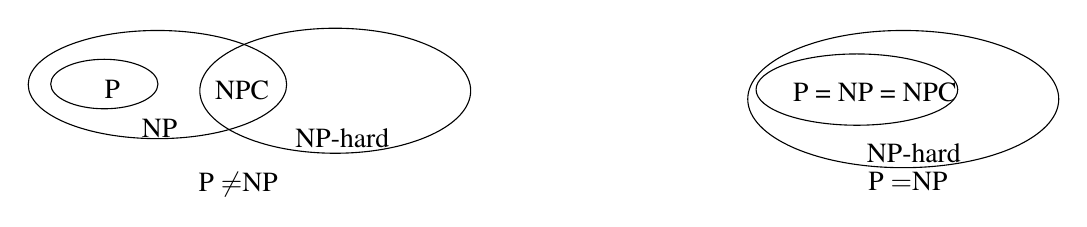
\begin{tikzpicture}[x=0.5pt,y=0.5pt,yscale=-1,xscale=1]
%uncomment if require: \path (0,124); %set diagram left start at 0, and has height of 124

%Shape: Ellipse [id:dp5973445750134718] 
\draw   (2.75,41.92) .. controls (2.75,20.33) and (44.56,2.83) .. (96.13,2.83) .. controls (147.69,2.83) and (189.5,20.33) .. (189.5,41.92) .. controls (189.5,63.5) and (147.69,81) .. (96.13,81) .. controls (44.56,81) and (2.75,63.5) .. (2.75,41.92) -- cycle ;
%Shape: Ellipse [id:dp8841818331933643] 
\draw   (19,41.54) .. controls (19,31.66) and (36.35,23.66) .. (57.75,23.66) .. controls (79.15,23.66) and (96.5,31.66) .. (96.5,41.54) .. controls (96.5,51.42) and (79.15,59.42) .. (57.75,59.42) .. controls (36.35,59.42) and (19,51.42) .. (19,41.54) -- cycle ;
%Shape: Ellipse [id:dp3401453478358991] 
\draw   (126.75,46.39) .. controls (126.75,21.44) and (170.57,1.21) .. (224.63,1.21) .. controls (278.68,1.21) and (322.5,21.44) .. (322.5,46.39) .. controls (322.5,71.33) and (278.68,91.56) .. (224.63,91.56) .. controls (170.57,91.56) and (126.75,71.33) .. (126.75,46.39) -- cycle ;
%Shape: Ellipse [id:dp5090440012854042] 
\draw   (528.75,45.55) .. controls (528.75,31.32) and (561.38,19.79) .. (601.63,19.79) .. controls (641.87,19.79) and (674.5,31.32) .. (674.5,45.55) .. controls (674.5,59.78) and (641.87,71.31) .. (601.63,71.31) .. controls (561.38,71.31) and (528.75,59.78) .. (528.75,45.55) -- cycle ;
%Shape: Ellipse [id:dp5250684881928416] 
\draw   (522.75,52.41) .. controls (522.75,25.03) and (573.06,2.83) .. (635.13,2.83) .. controls (697.19,2.83) and (747.5,25.03) .. (747.5,52.41) .. controls (747.5,79.8) and (697.19,102) .. (635.13,102) .. controls (573.06,102) and (522.75,79.8) .. (522.75,52.41) -- cycle ;

% Text Node
\draw (553.59,38.68) node [anchor=north west][inner sep=0.75pt]   [align=left] {P = NP = NPC};
% Text Node
\draw (608,103.5) node [anchor=north west][inner sep=0.75pt]   [align=left] {P $\displaystyle =$NP};
% Text Node
\draw (607,82.6) node [anchor=north west][inner sep=0.75pt]   [align=left] {NP-hard};
% Text Node
\draw (56,36.56) node [anchor=north west][inner sep=0.75pt]   [align=left] {P};
% Text Node
\draw (136,37.37) node [anchor=north west][inner sep=0.75pt]   [align=left] {NPC};
% Text Node
\draw (83,64.83) node [anchor=north west][inner sep=0.75pt]   [align=left] {NP};
% Text Node
\draw (124,103.5) node [anchor=north west][inner sep=0.75pt]   [align=left] {P $\displaystyle \neq $NP};
% Text Node
\draw (194,72.1) node [anchor=north west][inner sep=0.75pt]   [align=left] {NP-hard};


\end{tikzpicture}

}
\vspace*{-0.1cm}
\caption{Two possibilities among P, NP, NPC, and NP-hard.}
\label{fig:nphard}
\end{figure}


\end{document}
